\documentclass[twoside]{book}

% Packages required by doxygen
\usepackage{fixltx2e}
\usepackage{calc}
\usepackage{doxygen}
\usepackage[export]{adjustbox} % also loads graphicx
\usepackage{graphicx}
\usepackage[utf8]{inputenc}
\usepackage{makeidx}
\usepackage{multicol}
\usepackage{multirow}
\PassOptionsToPackage{warn}{textcomp}
\usepackage{textcomp}
\usepackage[nointegrals]{wasysym}
\usepackage[table]{xcolor}

% Font selection
\usepackage[T1]{fontenc}
\usepackage[scaled=.90]{helvet}
\usepackage{courier}
\usepackage{amssymb}
\usepackage{sectsty}
\renewcommand{\familydefault}{\sfdefault}
\allsectionsfont{%
  \fontseries{bc}\selectfont%
  \color{darkgray}%
}
\renewcommand{\DoxyLabelFont}{%
  \fontseries{bc}\selectfont%
  \color{darkgray}%
}
\newcommand{\+}{\discretionary{\mbox{\scriptsize$\hookleftarrow$}}{}{}}

% Page & text layout
\usepackage{geometry}
\geometry{%
  a4paper,%
  top=2.5cm,%
  bottom=2.5cm,%
  left=2.5cm,%
  right=2.5cm%
}
\tolerance=750
\hfuzz=15pt
\hbadness=750
\setlength{\emergencystretch}{15pt}
\setlength{\parindent}{0cm}
\setlength{\parskip}{3ex plus 2ex minus 2ex}
\makeatletter
\renewcommand{\paragraph}{%
  \@startsection{paragraph}{4}{0ex}{-1.0ex}{1.0ex}{%
    \normalfont\normalsize\bfseries\SS@parafont%
  }%
}
\renewcommand{\subparagraph}{%
  \@startsection{subparagraph}{5}{0ex}{-1.0ex}{1.0ex}{%
    \normalfont\normalsize\bfseries\SS@subparafont%
  }%
}
\makeatother

% Headers & footers
\usepackage{fancyhdr}
\pagestyle{fancyplain}
\fancyhead[LE]{\fancyplain{}{\bfseries\thepage}}
\fancyhead[CE]{\fancyplain{}{}}
\fancyhead[RE]{\fancyplain{}{\bfseries\leftmark}}
\fancyhead[LO]{\fancyplain{}{\bfseries\rightmark}}
\fancyhead[CO]{\fancyplain{}{}}
\fancyhead[RO]{\fancyplain{}{\bfseries\thepage}}
\fancyfoot[LE]{\fancyplain{}{}}
\fancyfoot[CE]{\fancyplain{}{}}
\fancyfoot[RE]{\fancyplain{}{\bfseries\scriptsize Generated by Doxygen }}
\fancyfoot[LO]{\fancyplain{}{\bfseries\scriptsize Generated by Doxygen }}
\fancyfoot[CO]{\fancyplain{}{}}
\fancyfoot[RO]{\fancyplain{}{}}
\renewcommand{\footrulewidth}{0.4pt}
\renewcommand{\chaptermark}[1]{%
  \markboth{#1}{}%
}
\renewcommand{\sectionmark}[1]{%
  \markright{\thesection\ #1}%
}

% Indices & bibliography
\usepackage{natbib}
\usepackage[titles]{tocloft}
\setcounter{tocdepth}{3}
\setcounter{secnumdepth}{5}
\makeindex

% Hyperlinks (required, but should be loaded last)
\usepackage{ifpdf}
\ifpdf
  \usepackage[pdftex,pagebackref=true]{hyperref}
\else
  \usepackage[ps2pdf,pagebackref=true]{hyperref}
\fi
\hypersetup{%
  colorlinks=true,%
  linkcolor=blue,%
  citecolor=blue,%
  unicode%
}

% Custom commands
\newcommand{\clearemptydoublepage}{%
  \newpage{\pagestyle{empty}\cleardoublepage}%
}

\usepackage{caption}
\captionsetup{labelsep=space,justification=centering,font={bf},singlelinecheck=off,skip=4pt,position=top}

%===== C O N T E N T S =====

\begin{document}

% Titlepage & ToC
\hypersetup{pageanchor=false,
             bookmarksnumbered=true,
             pdfencoding=unicode
            }
\pagenumbering{alph}
\begin{titlepage}
\vspace*{7cm}
\begin{center}%
{\Large My Project }\\
\vspace*{1cm}
{\large Generated by Doxygen 1.8.13}\\
\end{center}
\end{titlepage}
\clearemptydoublepage
\pagenumbering{roman}
\tableofcontents
\clearemptydoublepage
\pagenumbering{arabic}
\hypersetup{pageanchor=true}

%--- Begin generated contents ---
\chapter{Hierarchical Index}
\section{Class Hierarchy}
This inheritance list is sorted roughly, but not completely, alphabetically\+:\begin{DoxyCompactList}
\item \contentsline{section}{Point}{\pageref{class_point}}{}
\item \contentsline{section}{Poligono}{\pageref{class_poligono}}{}
\begin{DoxyCompactList}
\item \contentsline{section}{Retangulo}{\pageref{class_retangulo}}{}
\end{DoxyCompactList}
\end{DoxyCompactList}

\chapter{Class Index}
\section{Class List}
Here are the classes, structs, unions and interfaces with brief descriptions\+:\begin{DoxyCompactList}
\item\contentsline{section}{\hyperlink{classPoint}{Point} }{\pageref{classPoint}}{}
\item\contentsline{section}{\hyperlink{classPoligono}{Poligono} }{\pageref{classPoligono}}{}
\item\contentsline{section}{\hyperlink{classRetangulo}{Retangulo} }{\pageref{classRetangulo}}{}
\end{DoxyCompactList}

\chapter{Class Documentation}
\hypertarget{classPoint}{}\section{Point Class Reference}
\label{classPoint}\index{Point@{Point}}
\subsection*{Public Member Functions}
\begin{DoxyCompactItemize}
\item 
\mbox{\Hypertarget{classPoint_a06c32166c2ad9eac25799ef189b49683}\label{classPoint_a06c32166c2ad9eac25799ef189b49683}} 
{\bfseries Point} (float \+\_\+x=0, float \+\_\+y=0)
\item 
\mbox{\Hypertarget{classPoint_a428a1676e2fdec6753c42011a1d59d18}\label{classPoint_a428a1676e2fdec6753c42011a1d59d18}} 
void {\bfseries setX} (float \+\_\+x)
\item 
\mbox{\Hypertarget{classPoint_a9868c4601b0ea0c2d0de20fe41ee0e49}\label{classPoint_a9868c4601b0ea0c2d0de20fe41ee0e49}} 
void {\bfseries setY} (float \+\_\+y)
\item 
\mbox{\Hypertarget{classPoint_ab5385c6d9bfa841e641e4709fc9f14cc}\label{classPoint_ab5385c6d9bfa841e641e4709fc9f14cc}} 
void {\bfseries set\+XY} (float \+\_\+x, float \+\_\+y)
\item 
\mbox{\Hypertarget{classPoint_acc27466778cc87a662bba40268c4c0c8}\label{classPoint_acc27466778cc87a662bba40268c4c0c8}} 
float {\bfseries getX} ()
\item 
\mbox{\Hypertarget{classPoint_a3cccbca94719ddde353cce86ce0e2f64}\label{classPoint_a3cccbca94719ddde353cce86ce0e2f64}} 
float {\bfseries getY} ()
\item 
\mbox{\Hypertarget{classPoint_a6bcf8fd2524ecc4d5b6c1dc942d541a5}\label{classPoint_a6bcf8fd2524ecc4d5b6c1dc942d541a5}} 
void {\bfseries add} (\hyperlink{classPoint}{Point} p1)
\item 
\mbox{\Hypertarget{classPoint_af7d9e533f0030edf4ab28fdc0f12acd4}\label{classPoint_af7d9e533f0030edf4ab28fdc0f12acd4}} 
void {\bfseries sub} (\hyperlink{classPoint}{Point} p1)
\item 
\mbox{\Hypertarget{classPoint_a6233714649b03294a020827fb53eb8ad}\label{classPoint_a6233714649b03294a020827fb53eb8ad}} 
void {\bfseries norma} ()
\item 
\mbox{\Hypertarget{classPoint_ad9676e36f3444534b609e3c68422239a}\label{classPoint_ad9676e36f3444534b609e3c68422239a}} 
void {\bfseries translada} (float a, float b)
\item 
\mbox{\Hypertarget{classPoint_a1fb5c2501c27ab2cbc99d06c2a26a741}\label{classPoint_a1fb5c2501c27ab2cbc99d06c2a26a741}} 
void {\bfseries imprime} ()
\item 
\mbox{\Hypertarget{classPoint_a428a1676e2fdec6753c42011a1d59d18}\label{classPoint_a428a1676e2fdec6753c42011a1d59d18}} 
void {\bfseries setX} (float \+\_\+x)
\item 
\mbox{\Hypertarget{classPoint_a9868c4601b0ea0c2d0de20fe41ee0e49}\label{classPoint_a9868c4601b0ea0c2d0de20fe41ee0e49}} 
void {\bfseries setY} (float \+\_\+y)
\item 
\mbox{\Hypertarget{classPoint_ab5385c6d9bfa841e641e4709fc9f14cc}\label{classPoint_ab5385c6d9bfa841e641e4709fc9f14cc}} 
void {\bfseries set\+XY} (float \+\_\+x, float \+\_\+y)
\item 
\mbox{\Hypertarget{classPoint_acc27466778cc87a662bba40268c4c0c8}\label{classPoint_acc27466778cc87a662bba40268c4c0c8}} 
float {\bfseries getX} ()
\item 
\mbox{\Hypertarget{classPoint_a3cccbca94719ddde353cce86ce0e2f64}\label{classPoint_a3cccbca94719ddde353cce86ce0e2f64}} 
float {\bfseries getY} ()
\item 
\mbox{\Hypertarget{classPoint_a6bcf8fd2524ecc4d5b6c1dc942d541a5}\label{classPoint_a6bcf8fd2524ecc4d5b6c1dc942d541a5}} 
void {\bfseries add} (\hyperlink{classPoint}{Point} p1)
\item 
\mbox{\Hypertarget{classPoint_af7d9e533f0030edf4ab28fdc0f12acd4}\label{classPoint_af7d9e533f0030edf4ab28fdc0f12acd4}} 
void {\bfseries sub} (\hyperlink{classPoint}{Point} p1)
\item 
\mbox{\Hypertarget{classPoint_a6233714649b03294a020827fb53eb8ad}\label{classPoint_a6233714649b03294a020827fb53eb8ad}} 
void {\bfseries norma} ()
\item 
\mbox{\Hypertarget{classPoint_ad9676e36f3444534b609e3c68422239a}\label{classPoint_ad9676e36f3444534b609e3c68422239a}} 
void {\bfseries translada} (float a, float b)
\item 
\mbox{\Hypertarget{classPoint_a1fb5c2501c27ab2cbc99d06c2a26a741}\label{classPoint_a1fb5c2501c27ab2cbc99d06c2a26a741}} 
void {\bfseries imprime} ()
\end{DoxyCompactItemize}


The documentation for this class was generated from the following files\+:\begin{DoxyCompactItemize}
\item 
Point.\+h\item 
Point\+\_\+copy.\+h\item 
Point.\+cpp\end{DoxyCompactItemize}

\hypertarget{classPoligono}{}\section{Poligono Class Reference}
\label{classPoligono}\index{Poligono@{Poligono}}
Inheritance diagram for Poligono\+:\begin{figure}[H]
\begin{center}
\leavevmode
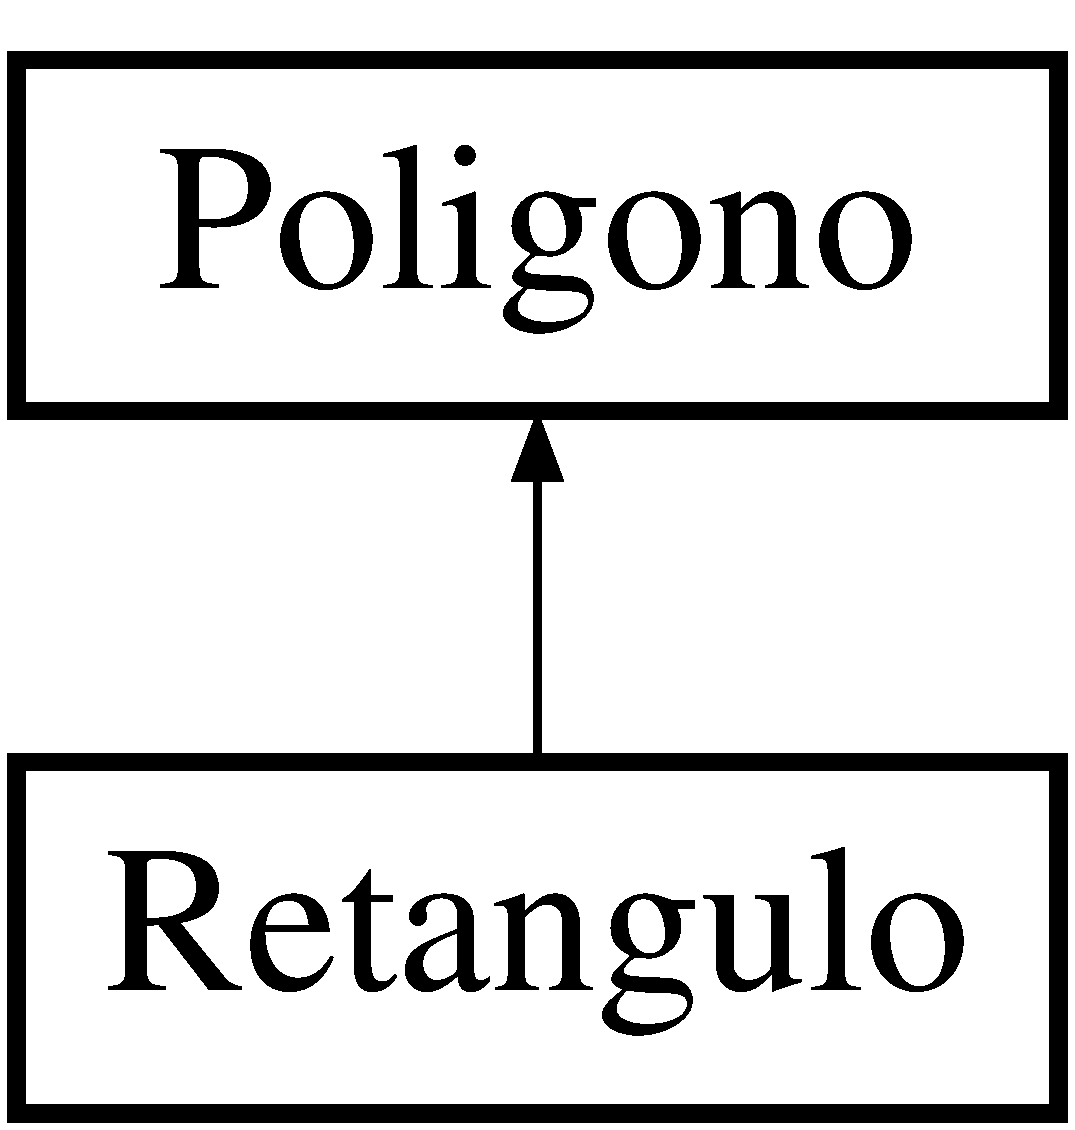
\includegraphics[height=2.000000cm]{classPoligono}
\end{center}
\end{figure}
\subsection*{Public Member Functions}
\begin{DoxyCompactItemize}
\item 
\mbox{\Hypertarget{classPoligono_a4d4cffe97d7190db1f8598b0f9f95763}\label{classPoligono_a4d4cffe97d7190db1f8598b0f9f95763}} 
void {\bfseries setN} (int \+\_\+n)
\item 
\mbox{\Hypertarget{classPoligono_a56257204345b9be3bb5d5fbe45ce63f1}\label{classPoligono_a56257204345b9be3bb5d5fbe45ce63f1}} 
int {\bfseries getN} (void)
\item 
\mbox{\Hypertarget{classPoligono_ae4e04e6cba0515395a9182cdb8ccb7dd}\label{classPoligono_ae4e04e6cba0515395a9182cdb8ccb7dd}} 
void {\bfseries set\+Vertice} (float \+\_\+x, float \+\_\+y, int i)
\item 
\mbox{\Hypertarget{classPoligono_a051cc49fca5417dbc8c6ba7a1edc2723}\label{classPoligono_a051cc49fca5417dbc8c6ba7a1edc2723}} 
float {\bfseries area\+Poligono} (void)
\item 
\mbox{\Hypertarget{classPoligono_ab37e1487cfe3360fa4f666dc917c6836}\label{classPoligono_ab37e1487cfe3360fa4f666dc917c6836}} 
void {\bfseries rotaciona\+Poligono} (\hyperlink{classPoint}{Point} ponto, double theta)
\item 
\mbox{\Hypertarget{classPoligono_a4d757f52ba9366ab13537fb19b363e1e}\label{classPoligono_a4d757f52ba9366ab13537fb19b363e1e}} 
void {\bfseries translada\+Poligono} (float a, float b)
\item 
\mbox{\Hypertarget{classPoligono_a87d58f9d4827793eaa811491cce097b0}\label{classPoligono_a87d58f9d4827793eaa811491cce097b0}} 
void {\bfseries imprime\+Poligono} ()
\end{DoxyCompactItemize}


The documentation for this class was generated from the following files\+:\begin{DoxyCompactItemize}
\item 
Poligono.\+h\item 
Poligono.\+cpp\end{DoxyCompactItemize}

\hypertarget{classRetangulo}{}\section{Retangulo Class Reference}
\label{classRetangulo}\index{Retangulo@{Retangulo}}
Inheritance diagram for Retangulo\+:\begin{figure}[H]
\begin{center}
\leavevmode
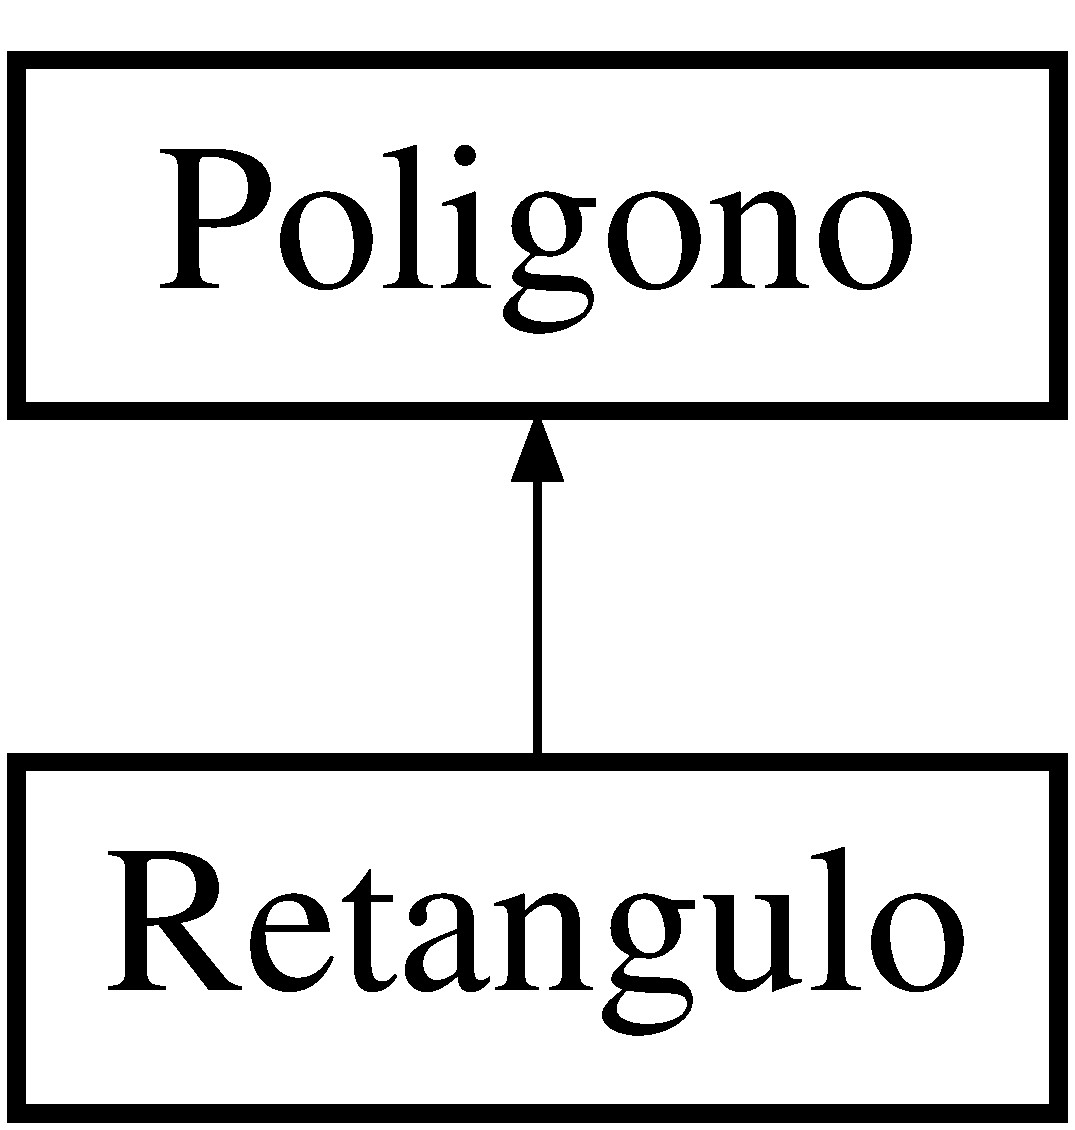
\includegraphics[height=2.000000cm]{classRetangulo}
\end{center}
\end{figure}
\subsection*{Public Member Functions}
\begin{DoxyCompactItemize}
\item 
\mbox{\Hypertarget{classRetangulo_a7bb0f3ead5f9b7610f3c7187a5a8c002}\label{classRetangulo_a7bb0f3ead5f9b7610f3c7187a5a8c002}} 
{\bfseries Retangulo} (float \+\_\+xr=0, float \+\_\+yr=0, float \+\_\+largura=1, float \+\_\+altura=1)
\item 
\mbox{\Hypertarget{classRetangulo_a9c332035e5f045f98b3da1549172acd4}\label{classRetangulo_a9c332035e5f045f98b3da1549172acd4}} 
float {\bfseries get\+Altura} (void)
\item 
\mbox{\Hypertarget{classRetangulo_a13f129bc990f54e6fba908cca70b2116}\label{classRetangulo_a13f129bc990f54e6fba908cca70b2116}} 
float {\bfseries get\+Largura} (void)
\end{DoxyCompactItemize}


The documentation for this class was generated from the following files\+:\begin{DoxyCompactItemize}
\item 
Retangulo.\+h\item 
Retangulo.\+cpp\end{DoxyCompactItemize}

%--- End generated contents ---

% Index
\backmatter
\newpage
\phantomsection
\clearemptydoublepage
\addcontentsline{toc}{chapter}{Index}
\printindex

\end{document}
